\documentclass[
size=17pt,
paper=smartboard,
mode=present,
display=slidesnotes,
style=paintings,
nopagebreaks,
blackslide,
fleqn]{powerdot}

% styles: sailor, paintings
% wj capsules prettybox
% mode = handout or present


\usepackage{amsmath,graphicx,color,amsfonts}
\usepackage[brazilian]{babel}
\usepackage[ruled,vlined,portuguese,portuguesekw]{algorithm2e}
\usepackage[utf8]{inputenc}
\newcommand{\palette}{Moitessier}


% palettes:
%    - sailor: Sea, River, Wine, Chocolate, Cocktail 
%    - paintings: Syndics, Skater, GoldenGate, Moitessier, PearlEarring, Lamentation, HolyWood, Europa, MayThird, Charon 

\newcommand{\cursopequeno}{EC01039 CG\underline{PI}}
\newcommand{\cursogrande}{\Large EC01039 -- Computação gráfica e \underline{processamento de imagem}}



\author{Ronaldo de Freitas Zampolo\\FCT-ITEC-UFPA}
\date{ERE 2020}


\DeclareMathOperator*{\mediana}{mediana}
\pdsetup{
	lf = {\cursopequeno},
	rf = {Restauração}, 
	cf = {\arabic{slide}~/~\pageref*{lastslide}},
	palette = {\palette}, 
	randomdots={false}
}

%opening
\title{\cursogrande\\ \vspace{1cm}Restauração e imagens}
\author{Ronaldo de Freitas Zampolo\\FCT-ITEC-UFPA}
%\date{ }

\begin{document}
   \maketitle[randomdots={false}]
   \begin{slide}{Agenda}
      \tableofcontents[content=sections]
   \end{slide}

\section[ slide = true]{Introdução}
   \begin{slide}[toc=]{Conceitos iniciais}
      \begin{itemize}
       \item Objetivo
	       \begin{itemize}
		       \item Melhorar a qualidade de uma imagem
		       \item Qualidade em qual sentido? 
			       \begin{itemize}
				       \item Critérios objetivos: métrica, equação
				       \item Critérios subjetivos: opinião de pessoas
				       \item Critérios objetivos perceptuais: modelo da percepção humana da qualidade visual
			       \end{itemize}
	       \end{itemize}
       \item Restauração \emph{versus} Realce 
	       \begin{itemize}
		       \item Realce: qualidade estética/subjetiva (alguém olha e avalia)
		       \item Restauração: há um modelo matemático para o sistema de formação de imagem e a definição de um ótimo matemático
	       \end{itemize}
       \end{itemize}
   \end{slide}

\section[slide=true]{Modelo dos sistemas de formação e restauração}
\begin{slide}[toc=]{Modelos de formação/degradação e restauração}
	\begin{itemize}
		\item Sistemas de degradação e restauração
			\begin{center}
				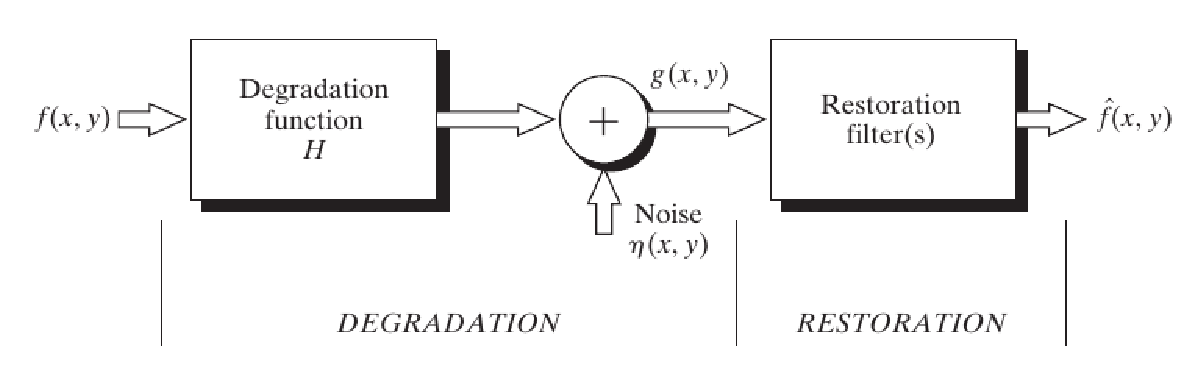
\includegraphics[width=0.55\textwidth]{figs/5-01}
			\end{center}
		\item Modelo de degradação:
			\begin{align*}
				g(x,y) &= h(x,y)\ast f(x,y) + \eta(x,y)\\
				G(u,v) &= H(u,v) F(u,v) + N(u,v)
			\end{align*}
		\item Modelo de restauração:
			\begin{align*}
				\hat f(x,y) &= R\{g(x,y)\}\\
					    &= R\{h(x,y)\ast f(x,y) + \eta(x,y)\}
			\end{align*}
	\end{itemize}
\end{slide}
   
\section[slide=true]{Ruído}
\begin{slide}[toc=]{Fontes de ruído}
	Algumas fontes de ruído:
	\begin{itemize}[type=1]
		\item Ruído térmico: 
			\begin{itemize}
				\item Partículas carregadas nos foto-sensores.
				\item Inerente à agitação devido à temperatura.
			\end{itemize}
		\item Intensidade de iluminação: 
			\begin{itemize}
				\item Ruído proporcional à intensidade luminosa.
				\item Modelo AWGN não se aplica (ruído multiplicativo).
			\end{itemize}
		\item Interferências no processo de transmissão.
	\end{itemize}
\end{slide}
     
\begin{slide}[toc=]{Tipos de ruído}
Ruído aditivo do tipo branco:
	\twocolumn{
		\begin{itemize}
			\item Ruído gaussiano:
				\begin{equation*}
					p(z)=\frac{1}{\sqrt{2\pi}}\exp\left\{-\frac{(z-\bar z)^2}{2\sigma ^2}\right\}
				\end{equation*}
				\vspace{0.5cm}
				\begin{figure}[b!]
					\centering
					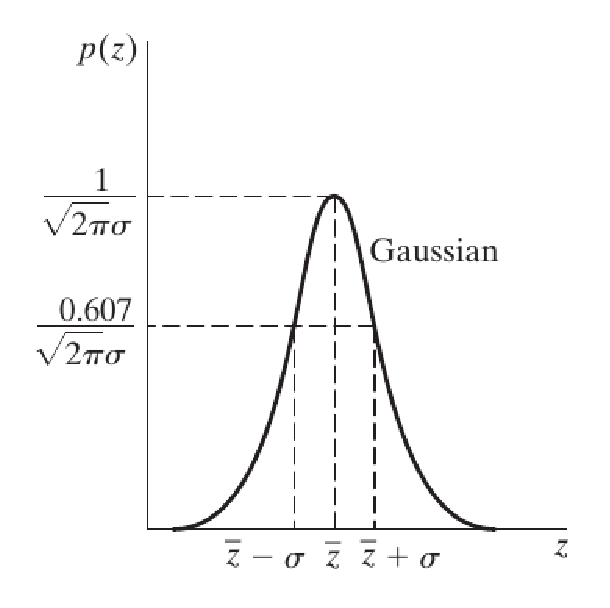
\includegraphics[width=0.6\textwidth]{figs/5-02a}
				\end{figure}
		\end{itemize}}
		{
		\begin{itemize}
			\item Ruído Rayleigh:
				\begin{equation*}
					p(z)=\begin{cases}
						\frac{2}{b}(z-a)\exp\left\{-\frac{(z-a)^2}{b}\right\}, & z\geq a\\
						0, & z<a
					\end{cases}
				\end{equation*}
				\begin{figure}[b!]
					\centering
					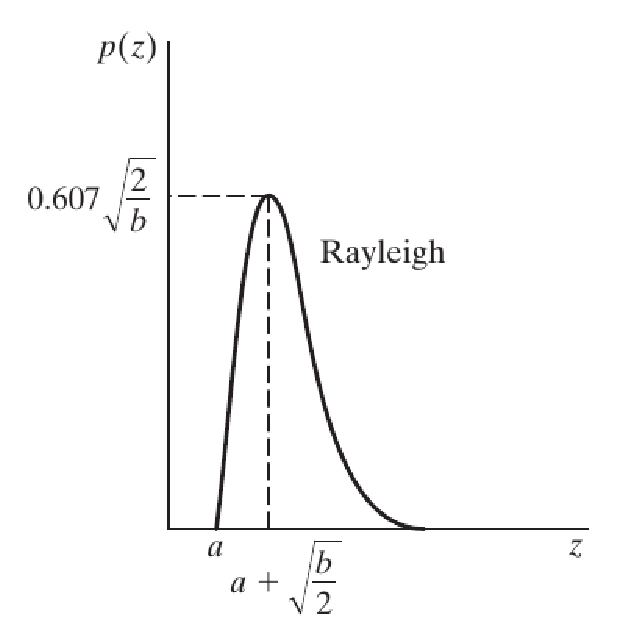
\includegraphics[width=0.6\textwidth]{figs/5-02b}
				\end{figure}
		\end{itemize}}
\end{slide}

\begin{slide}[toc=]{Tipos de ruído}
Ruído aditivo do tipo branco:
	\twocolumn{
		\begin{itemize}
			\item Ruído Erlang (Gama):
				\begin{align*}
					p(z)&=\begin{cases}
						\frac{a^bz^{b-1}}{(b-1)!}(z-a)\exp\left\{-az\right\}, & z\geq 0\\
						0, & z<0
					\end{cases}\\
					&a>0, \quad b \in \mathbb{N}^\ast
				\end{align*}
				%\vspace{0.5cm}
				\begin{figure}[b!]
					\centering
					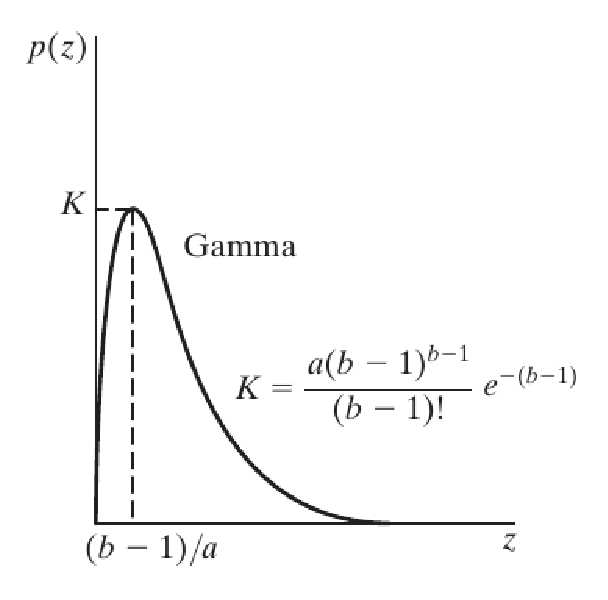
\includegraphics[width=0.6\textwidth]{figs/5-02c}
				\end{figure}
		\end{itemize}}
		{
		\begin{itemize}
			\item Ruído exponencial:
				\begin{align*}
					p(z)&=\begin{cases}
						a\exp\left\{-az\right\}, & z\geq 0\\
						0, & z<a
					\end{cases}\\
					& a>0
				\end{align*}
				\begin{figure}[b!]
					\centering
					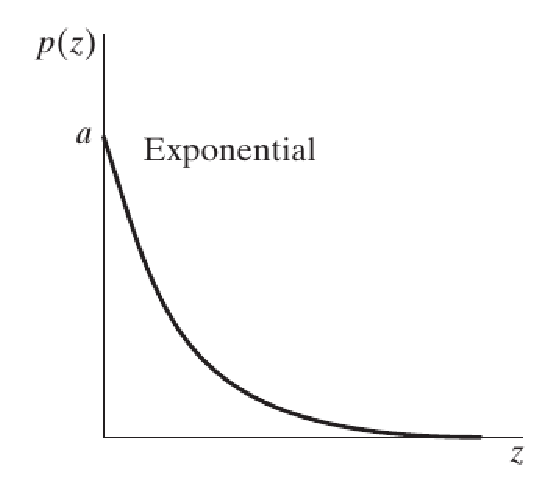
\includegraphics[width=0.6\textwidth]{figs/5-02d}
				\end{figure}
		\end{itemize}}
\end{slide}

\begin{slide}[toc=]{Tipos de ruído}
Ruído aditivo do tipo branco:
	\twocolumn{
		\begin{itemize}
			\item Ruído uniforme:
				\begin{equation*}
					p(z)=\begin{cases}
						\frac{1}{(b-a)}, & a\leq z\leq b\\
						0, & \text{outro caso}
					\end{cases}
				\end{equation*}
				\vspace{0.8cm}
				\begin{figure}[b!]
					\centering
					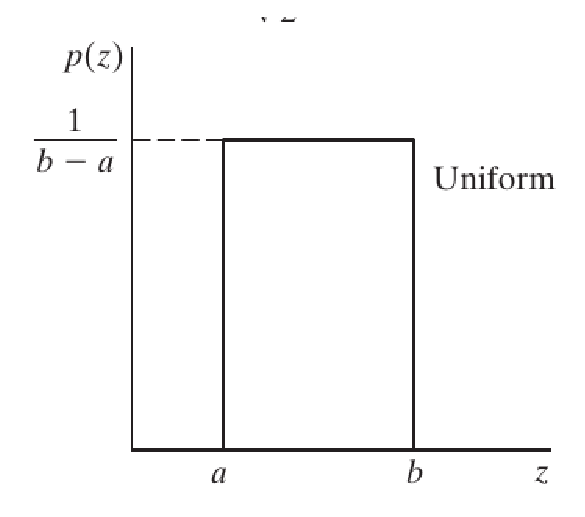
\includegraphics[width=0.6\textwidth]{figs/5-02e}
				\end{figure}
		\end{itemize}}
		{
		\begin{itemize}
			\item Ruído impulsivo (sal e pimenta):
				\begin{equation*}
					p(z)=\begin{cases}
						P_a, & z=a\\
						P_b, & z=b\\
						0, & \text{outro caso}
					\end{cases}
				\end{equation*}
				\begin{figure}[b!]
					\centering
					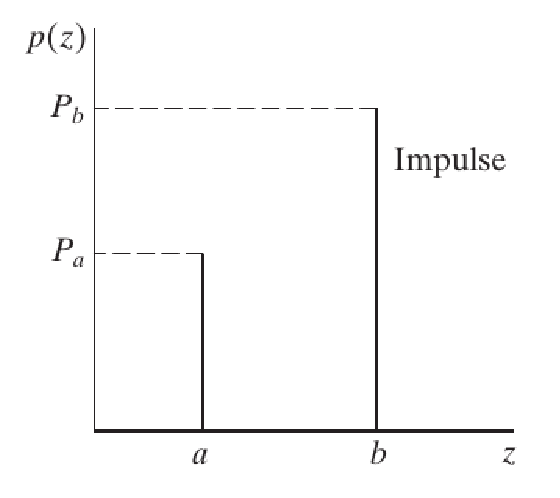
\includegraphics[width=0.6\textwidth]{figs/5-02f}
				\end{figure}
		\end{itemize}}
\end{slide}

\begin{slide}[toc=]{Uso do histograma na identificação de ruído aditivo}
	\twocolumn{
	\begin{itemize}
		\item Imagem de teste (sintética)
			\begin{center}
				
\includegraphics[width=0.8\textwidth]{figs/5-03}
			\end{center}
	\end{itemize}}
        {
	\begin{itemize}
		\item Procedimento:
			\begin{itemize}
				\item Adiciona ruído de determinado tipo à imagem de teste
				\item Calcula e exibe o histograma
				\item Compara com as funções de densidade de probabilidade
				\item Identifica o tipo por semelhança
			\end{itemize}
	\end{itemize}
	}
\end{slide}
      
\begin{slide}[toc=]{Uso do histograma na identificação de ruído aditivo}
Exemplos:
	\begin{center}
		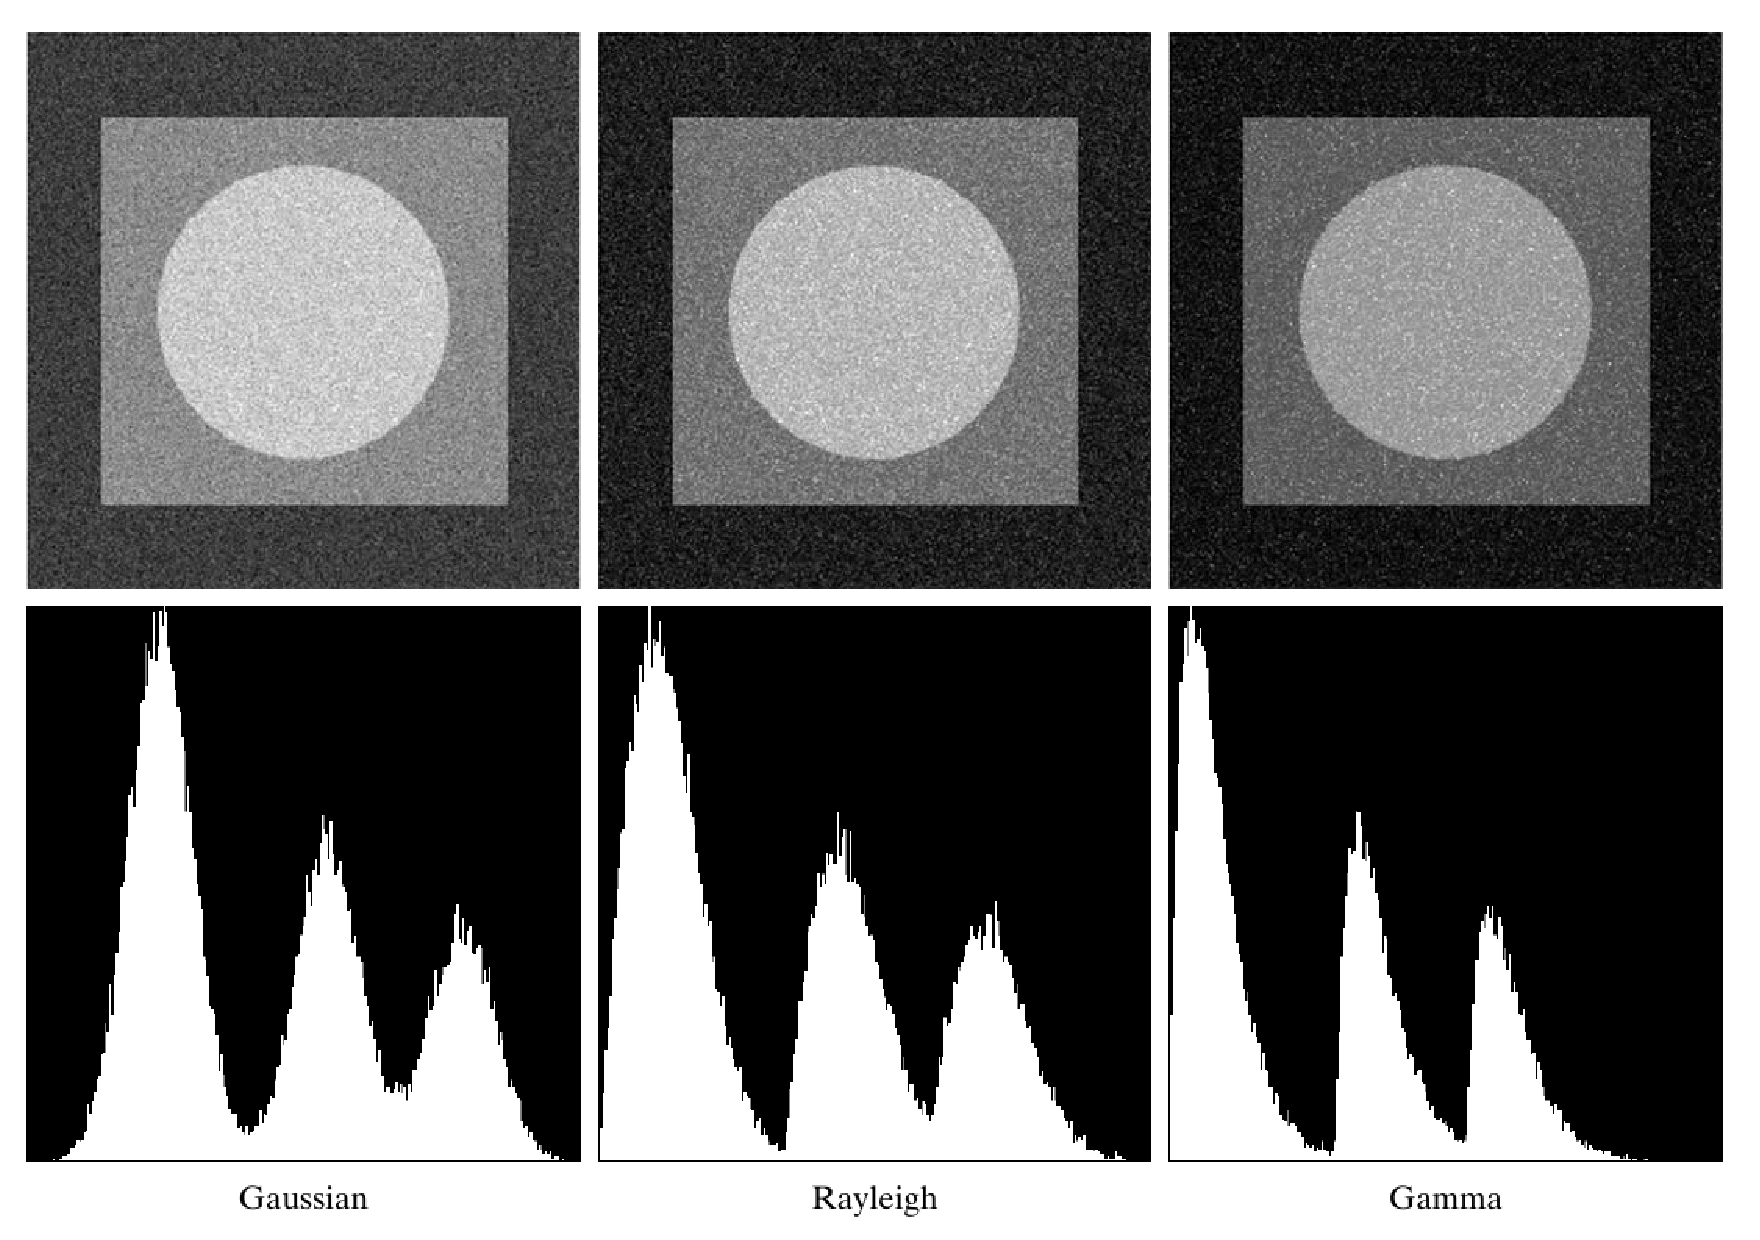
\includegraphics[width=0.7\textwidth]{figs/5-04a}
	\end{center}
\end{slide}

\begin{slide}[toc=]{Uso do histograma na identificação de ruído aditivo}
Exemplos:
	\begin{center}
		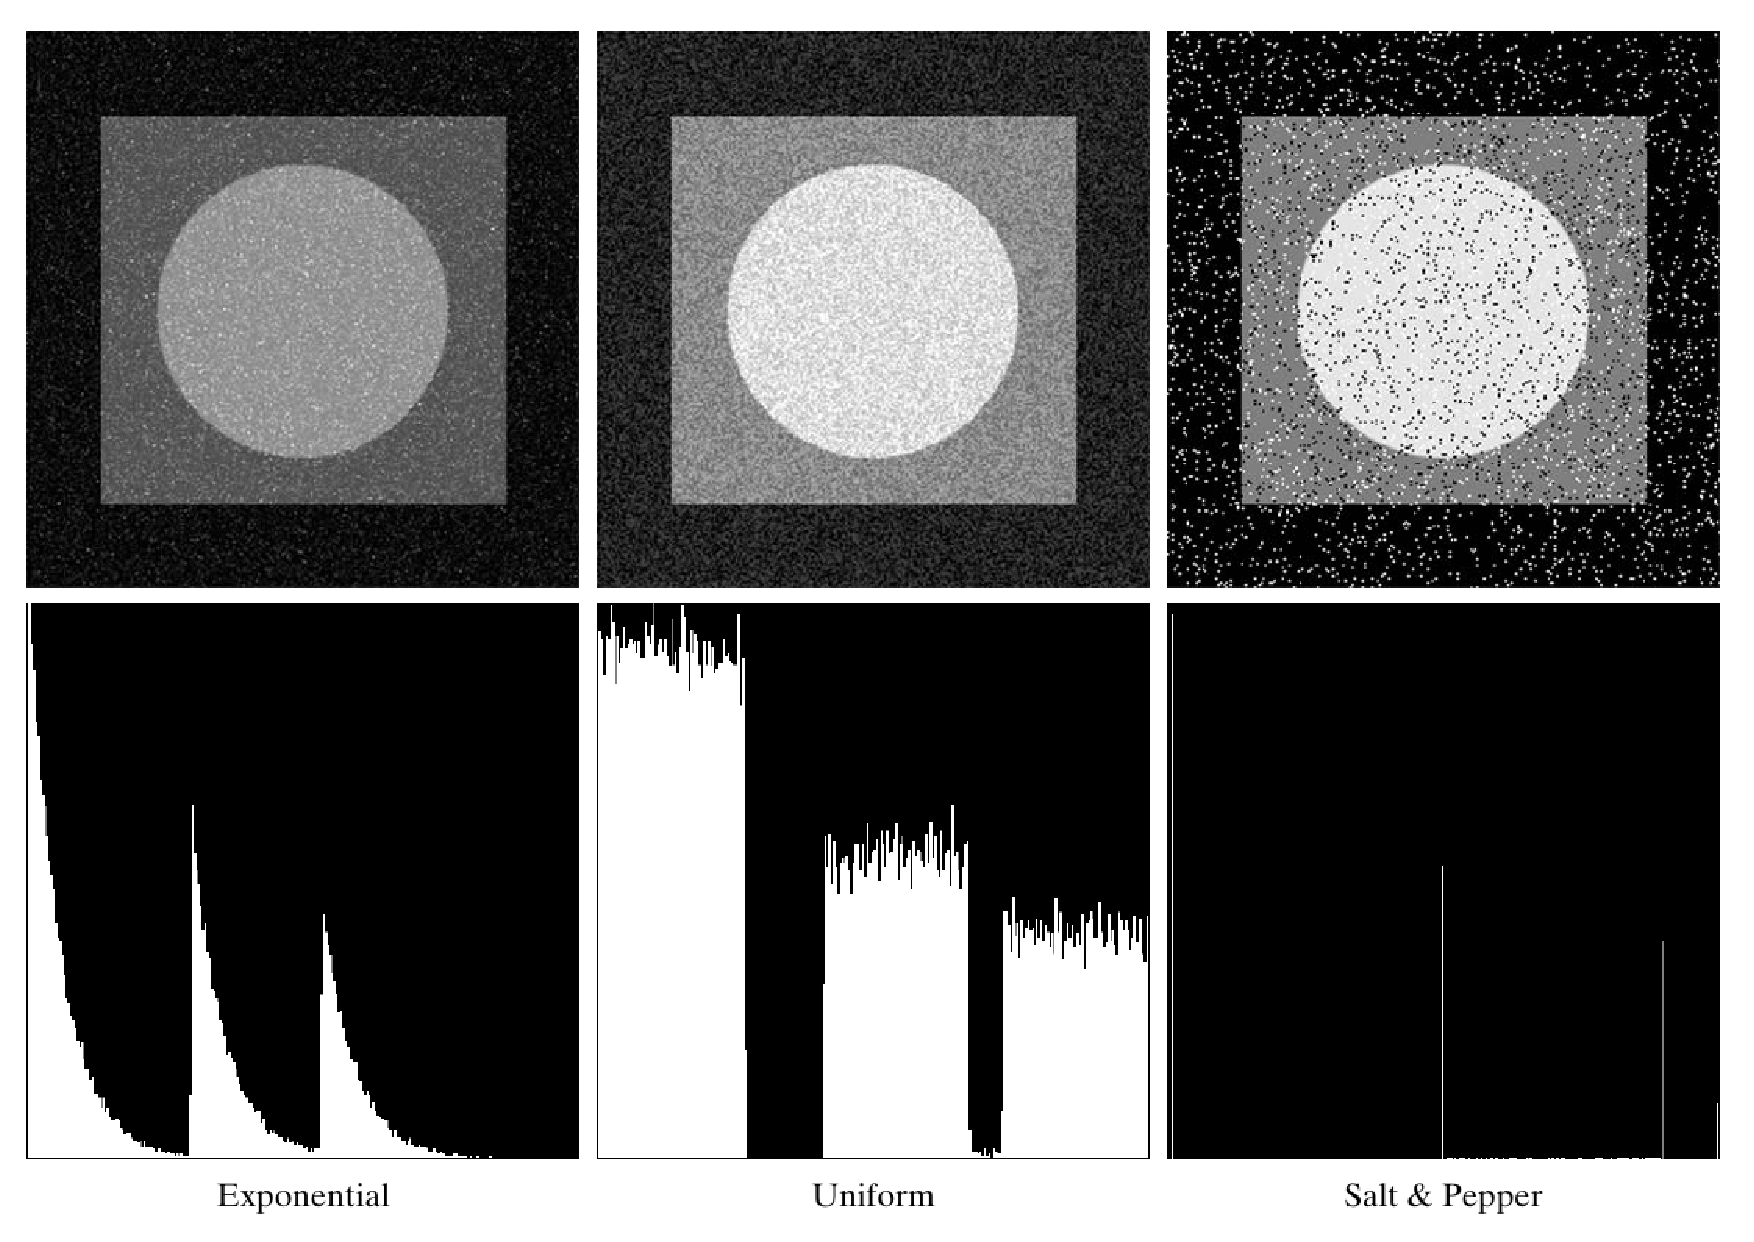
\includegraphics[width=0.7\textwidth]{figs/5-04b}
	\end{center}
\end{slide}
      
\begin{slide}[toc=]{Ruído periódico}
O ruído periódico mostra-se de maneira clara no domínio espectral !
	\begin{center}
		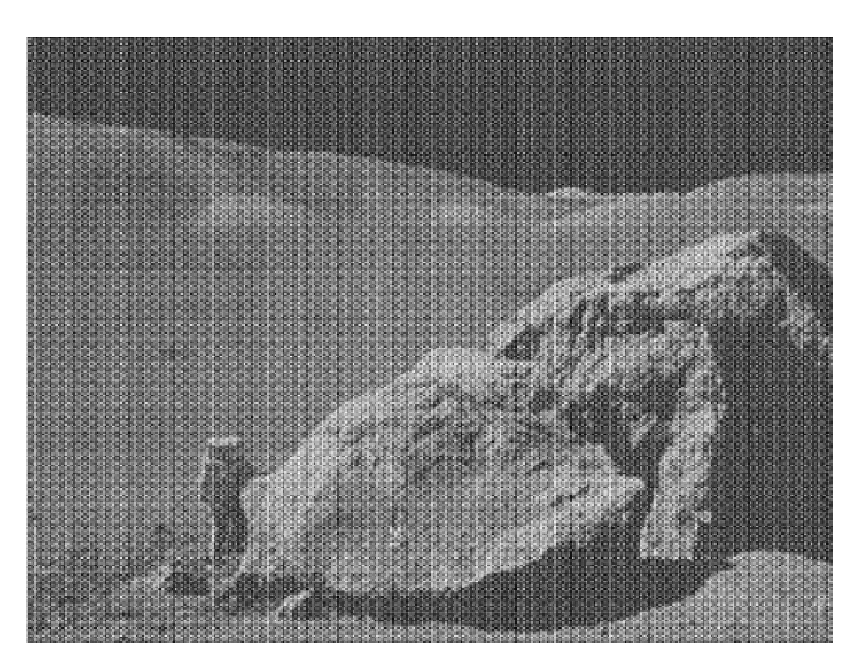
\includegraphics[width=0.45\textwidth]{figs/5-05a}
		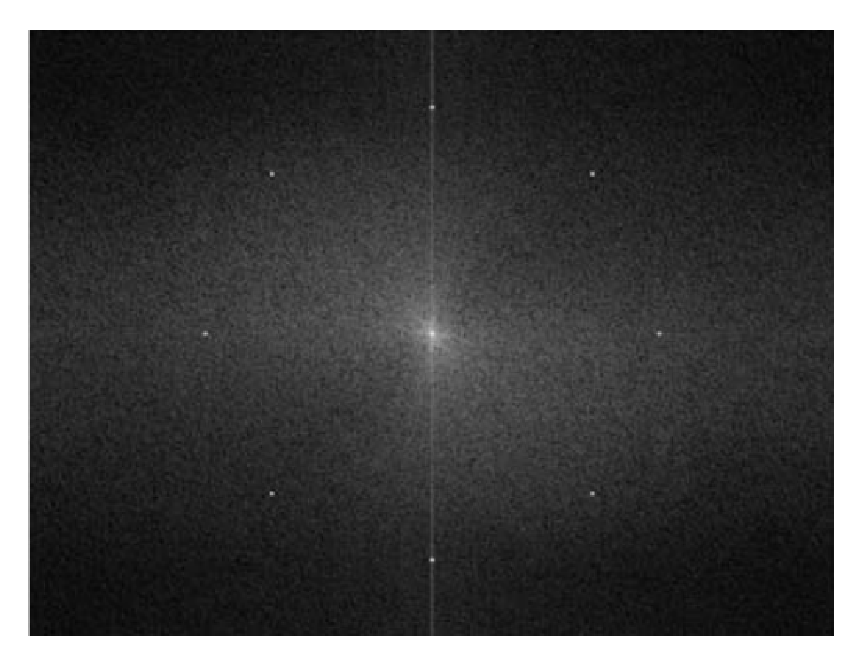
\includegraphics[width=0.45\textwidth]{figs/5-05b}
	\end{center}
\end{slide}

\section[slide=true]{Restauração em presença de ruído somente}
\begin{slide}{Introdução}
	\begin{itemize}
		\item A imagem é degradada apenas por ruído
		\item Não há efeitos de distorção em frequência
		\item Modelo de degradação:
			\begin{itemize}
				\item Domínio espacial:
					\begin{equation*}
						g(x,y) = f(x,y) + \eta(x,y)
					\end{equation*}
				\item Domínio da frequência:
					\begin{equation*}
						G(u,v) = F(u,v) + N(u,v)
					\end{equation*}
			\end{itemize}
	\end{itemize}
\end{slide}

\begin{slide}{Filtragem espacial}
	Filtros de média\vspace{0.5cm}
	\twocolumn{
		\begin{itemize}
			\item Média aritmética
				\begin{equation*}
					\hat f(x,y) = \frac{1}{mn} \sum_{(s,t)\in S_{xy}} g(s,t)
				\end{equation*}
			\item Média geométrica
				\begin{equation*}
					\hat f(x,y) =  \left [ \prod_{(s,t)\in S_{xy}} g(s,t) \right ]^\frac{1}{mn}
				\end{equation*}
				\footnotesize{Tende a perder menos detalhes que o filtro de média aritmética.}
		\end{itemize}
	}{
		
		\begin{itemize}
			\item Média harmônica
				\begin{equation*}
					\hat f(x,y) =  \frac{mn}{\sum_{(s,t)\in S_{xy}} \frac{1}{g(s,t)}}
				\end{equation*}
				{\footnotesize{Lida bem com ruído do tipo sal; falha para ruído do tipo pimenta; ok para outros tipos de ruído.}}
			\item Média contra-harmônica.
				\begin{equation*}
					\hat f(x,y) =  \frac{\sum_{(s,t)\in S_{xy}} g(s,t)^{Q+1}}{\sum_{(s,t)\in S_{xy}} g(s,t)^{Q}}
				\end{equation*}
				\footnotesize{Funciona com ruídos do tipo sal ($Q<0$) e pimenta ($Q>0$).}
		\end{itemize}
	}
\end{slide}

\begin{slide}{Filtragem espacial}
	Filtros de média: resultados\\
	\centering
	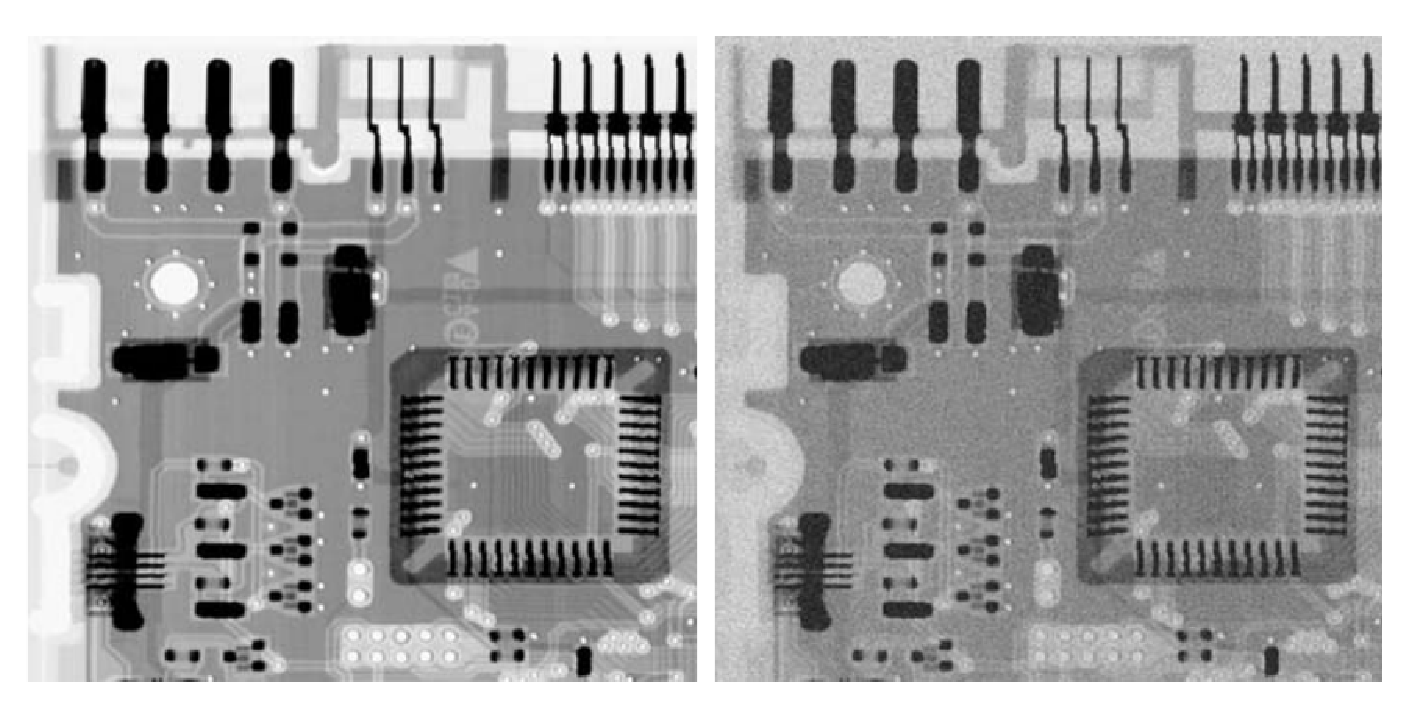
\includegraphics[width=0.5\textwidth]{figs/5-7ab}\\
	\tiny{(a)\hspace{4cm} (b)}\\
	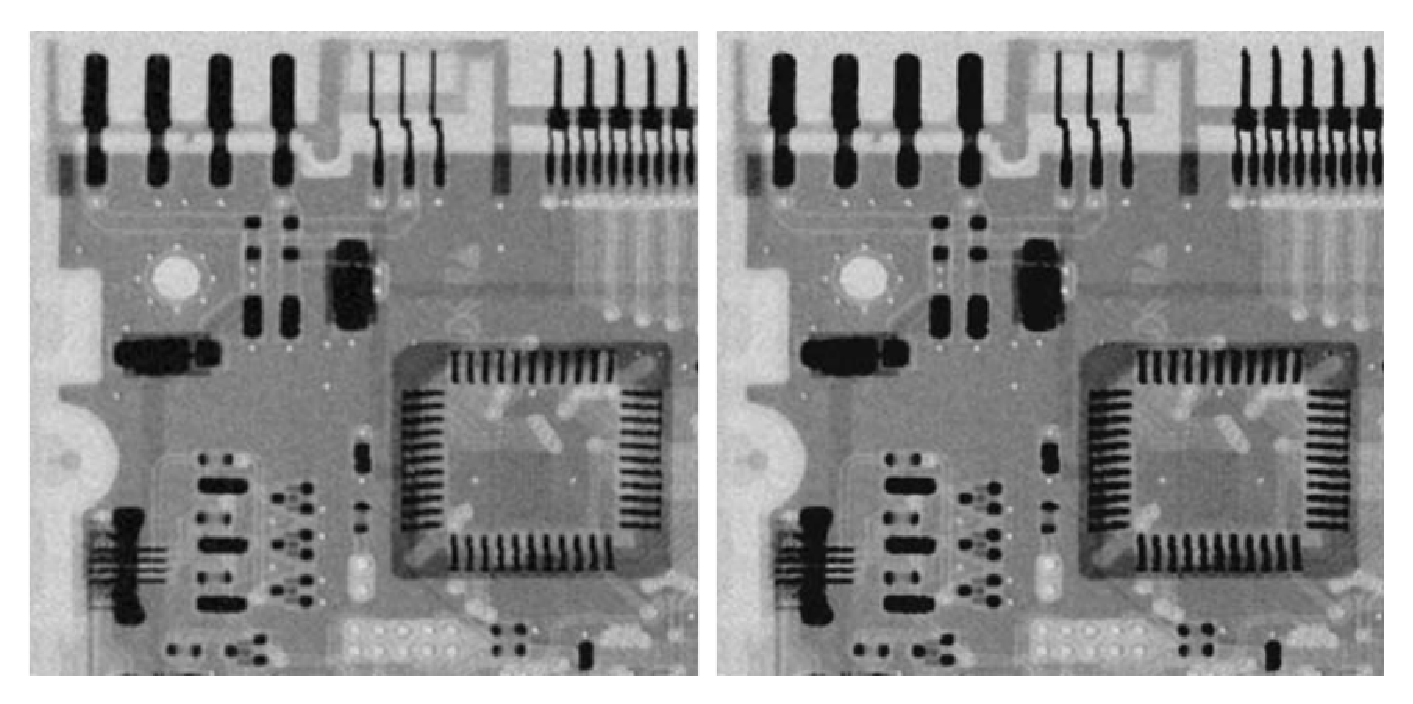
\includegraphics[width=0.5\textwidth]{figs/5-7cd}\\
	\tiny{(c)\hspace{4cm} (d)}\\
	\tiny{(a) imagem original; (b) imagem degradada por AWGN; (c) restauração por média aritmética (filtro 3$\times$3); (d) restauração por média geométrica (filtro 3$\times$3).}
\end{slide}
\begin{slide}{Filtragem espacial}
	Filtros de média: resultados\\
	\centering
	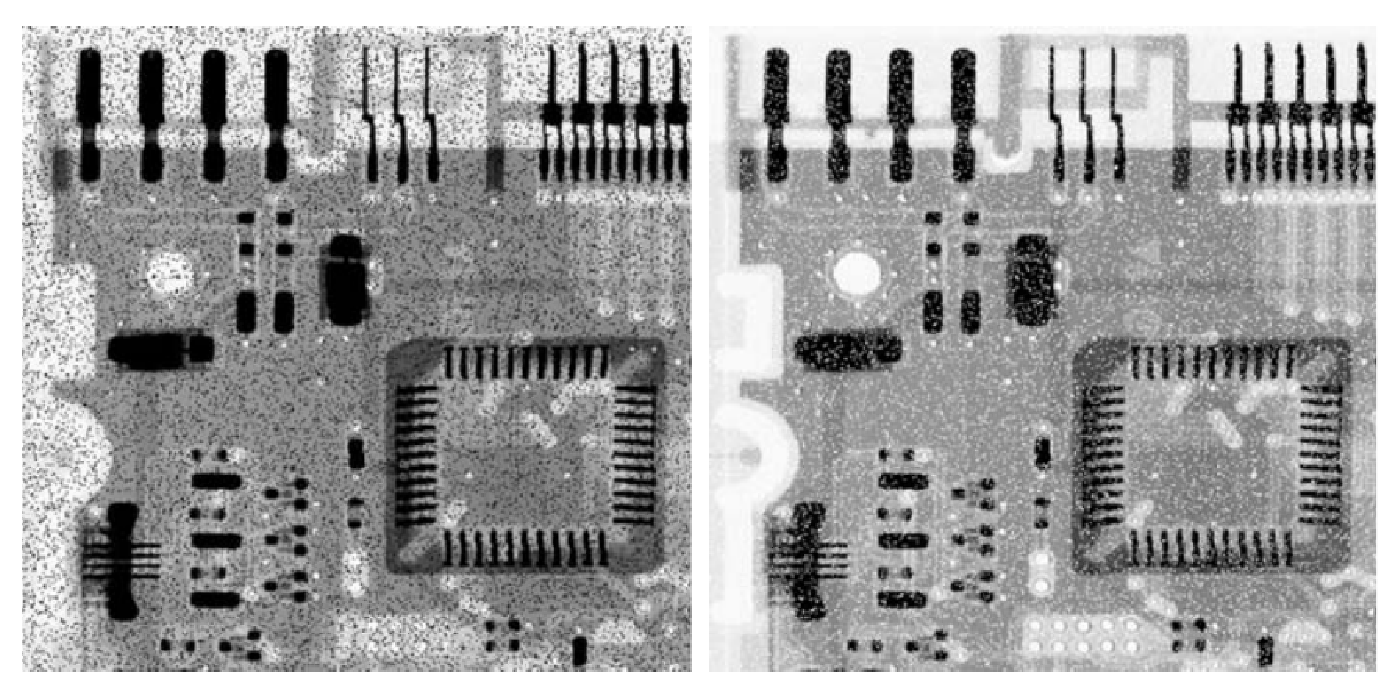
\includegraphics[width=0.5\textwidth]{figs/5-8ab}\\
	\tiny{(a)\hspace{4cm} (b)}\\
	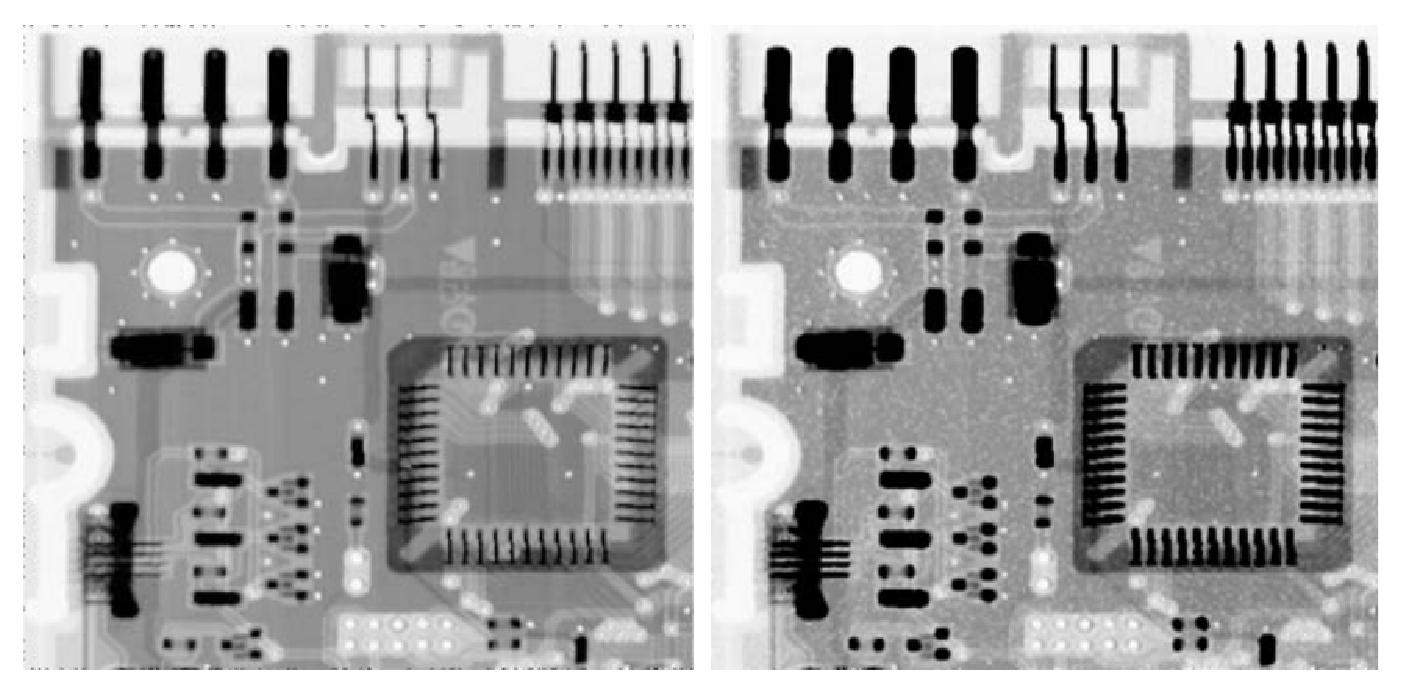
\includegraphics[width=0.5\textwidth]{figs/5-8cd}\\
	\tiny{(c)\hspace{4cm} (d)}\\
	\tiny{(a) imagem com ruído pimenta (probabilidade de 0,1); (b) imagem com ruído sal (probabilidade 0,1); (c) restauração de (a) com média contra-harmônica ($Q = 1,5$); (d) restauração de (b) com  média contra-harmônica ($Q=-1,5$).}
\end{slide}

\begin{slide}{Filtros de estatística de ordem}
	\twocolumn
	{
		\begin{itemize}
			\item Filtro de mediana
				\begin{equation*}
					\hat f(x,y) = \mediana_{(s,t)\in S_{xy} }g(s,t)
				\end{equation*}
			\item Filtro de mínimo
				\begin{equation*}
					\hat f(x,y) = \min_{(s,t)\in S_{xy} }g(s,t)
				\end{equation*}
			\item Filtro de máximo
				\begin{equation*}
					\hat f(x,y) = \max_{(s,t)\in S_{xy} }g(s,t)
				\end{equation*}
		\end{itemize}
	}
	{
		\begin{itemize}
			\item Filtro de ponto médio
				\begin{equation*}
					\hat f(x,y) = \frac{1}{2}\left [\min_{(s,t)\in S_{xy} }g(s,t)+\max_{(s,t)\in S_{xy} }g(s,t)\right ]
				\end{equation*}
			\item Filtro de média alfa cortada
				\begin{equation*}
					\hat f(x,y) = \frac{1}{mn-d}\sum_{(x,y)\in S_{xy}}g_r(s,t)
				\end{equation*}
				onde $g_r$ corresponde a $g$ em $S_{xy}$ com eliminação dos $d/2$ pixels de menor valor e dos $d/2$ pixels de maior valor.
		\end{itemize}

	}
\end{slide}

\begin{slide}{Filtros adaptativos}
	\begin{itemize}
		\item Objetivo: redução de ruído adaptado às características locais de uma imagem
		\item Comportamento desejado:
			\twocolumn{
			\begin{itemize}
				\item Se $\sigma^2_\eta =0$,
					\begin{equation*}
						\hat f(x,y) = g(x,y)
					\end{equation*}

				\item Se $\sigma^2_L = \sigma^2_\eta$,
					\begin{align*}
						\hat f(x,y)=&\frac{1}{mn}\sum_{(x,y)\in S_{xy}}g(s,t)\\
						=& m_L
					\end{align*}
					onde $\sigma_L^2$ é a variância da imagem original em $S_{xy}$.
			\end{itemize}
					}{
						\begin{itemize}
				\item Se $\sigma_L^2>\sigma_\eta^2$,
					\begin{equation*}
						\hat f(x,y) \approx g(x,y)
					\end{equation*}
				\item Aproximação do comportamento desejado:
					\begin{equation*}
						\hat f(x,y) = g(x,y) - \frac{\sigma_\eta^2}{\sigma_L^2}\left [ g(x,y) - m_L \right ]
					\end{equation*}
			\end{itemize}}
	\end{itemize}
\end{slide}

\begin{slide}{Filtro adaptativo de mediana}
	\begin{itemize}
		\item Objetivo: maior preservação de detalhes que no filtro de mediana convencional
			\footnotesize{
			\begin{algorithm}[H]
				\DontPrintSemicolon
				%\KwResult{Write here the result }
				\SetKwInOut{Input}{input}\SetKwInOut{Output}{output}
				\Input{Imagem degradada $g$, $S_\text{max}$, $(x,y)$, tamanho inicial de $S_{xy}$}
				\Output{$\hat f(x,y)$}
				\BlankLine
				%reinicia tamanho de $S_{xy}$\;
				\nlset{inicio}Define $S_{xy}$\;\label{ret}
				$z_\text{min} \leftarrow $ valor mínimo em $S_{xy}$\;
				$z_\text{max} \leftarrow  $ valor máximo em $S_{xy}$\;
				$z_\text{med} \leftarrow $ mediana em $S_{xy}$\;
				$z_{xy} \leftarrow g(x,y)$\;
				\BlankLine
				$A_1 \leftarrow z_\text{med} - z_\text{min}$\;
				$A_2 \leftarrow z_\text{med} - z_\text{max}$\;
				\If{$A_1>0\text{ E }A_2<0$}{
					$B_1 \leftarrow z_{xy} - z_\text{min}$\;
					$B_2 \leftarrow z_{xy} - z_\text{max}$\;
					\lIf{$B_1>0\text{ E }B_2<0$}{
						Retorna $z_\text{med}$
					}
				}
				\Else{
					Aumenta o tamanho de $S_{xy}$\;
					\lIf{$S_{xy}\leq S_\text{max}$}{
						Volta para~\ref{ret}
					}
					\lElse{
						Retorna $z_\text{med}$
					}
				}

					
				
				\caption{\footnotesize Filtragem adaptativa de mediana}
			\end{algorithm}}
	\end{itemize}
\end{slide}

\end{document}
